\section*{JPEG Compression}

\begin{itemize}
  \item Stands for Joint Photographic Experts Group
  \item JPEG compression is used with .jpg and can be embedded in
    .tiff and .eps files.
  \item Used on 24-bit color files.
  \item Works well on photographic images.
  \item Although it is a lossy compression technique, it yields an
    excellent quality image with high compression rates.
\end{itemize}

\subsection*{JPEG Compression Steps}

\begin{enumerate}

  \item (Optionally) If the color is represented in RGB mode,
    translate it to YUV.
  \item Divide the file into $8 \times 8$ blocks.
  \item Transform the pixel information from the spatial domain to
    the frequency domain with the \textbf{Discrete Cosine Transform}.
  \item Quantize the resulting values by \textbf{dividing each coefficient
    by an integer value} and rounding off to the \textbf{nearest integer}.
  \item Look at the resulting coefficients in a zigzag order. Do a
    \textbf{run-length encoding} of the coefficients ordered in this manner.
  \item Follow by \textbf{Huffman coding}.

\end{enumerate}

\subsection*{RGB to YUV Conversion}

There are several formulas, depending on the target monitor. A common one:

\begin{fleqn}[1.5em]
  \begin{flalign*}
    & Y = 0.299 \times R +   0.587 \times G +   0.114 \times B\\[0.5em]
    & U = -0.1687 \times R –   0.3313\times G + 0.5 \times B + 128\\[0.5em]
    & V = 0.5 \times R –   0.4187 \times G – 0.813 \times B + 128
  \end{flalign*}
\end{fleqn}

\textbf{Important Info:}

\begin{itemize}
  \item \textbf{Not required for JPEG}, but gives better compression rate.
  \item Why? The human eye is less sensitive to chrominance than luminance.
\end{itemize}

\subsection*{Discrete Cosine Transform (DCT)}

Spatial domain $\rightarrow$ frequency domain, like Fourier.

\begin{itemize}
  \item The spatial domain shows the amplitude of the color as you
    move through space
  \item The frequency domain shows how quickly the amplitude of the
    color is changing from one pixel to the next in an image file.
  \item Why frequency domain? Human eye is not very sensitive to high
    frequency changes; much of the high frequency data can be discarded
\end{itemize}

\begin{fleqn}[1.5em]
  \begin{gather*}
    \mathrm{DCT}_{u v}
    =
    \frac{1}{\sqrt{2N}}
    \,C_{u}C_{v}
    \sum_{x=0}^{N-1}\sum_{y=0}^{N-1}
    p_{x y}\\
    \hspace{8em}
    \cos\!\!\bigg[\frac{(2x+1)\,u\pi}{2N}\bigg]
    \cos\!\!\bigg[\frac{(2y+1)\,v\pi}{2N}\bigg]
  \end{gather*}

  \begin{gather*}
    C_{u}C_{v}=
    \begin{cases}
      \dfrac{1}{\sqrt{2}},&u,v=0,\\[6pt]
      1,&\text{otherwise.}
    \end{cases}
  \end{gather*}
\end{fleqn}

\subsection*{Zigzag Order}

\begin{figure}[H]
  \centering
  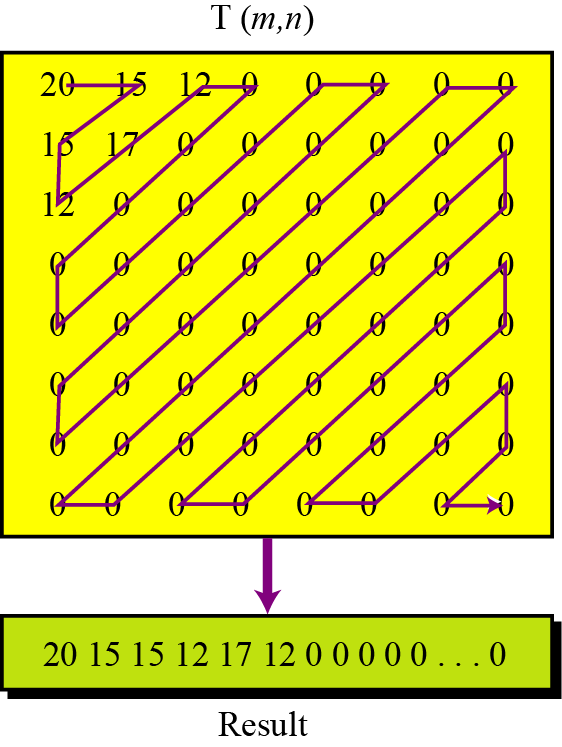
\includegraphics[width=0.7\linewidth]{images/zigzag.png}
  \caption{Reading Order of DCT Coefficients}
\end{figure}


\subsection*{Run-Length Encoding}

Converts a sequence of repeated values into a single value and a count.

\begin{figure}[H]
  \centering
  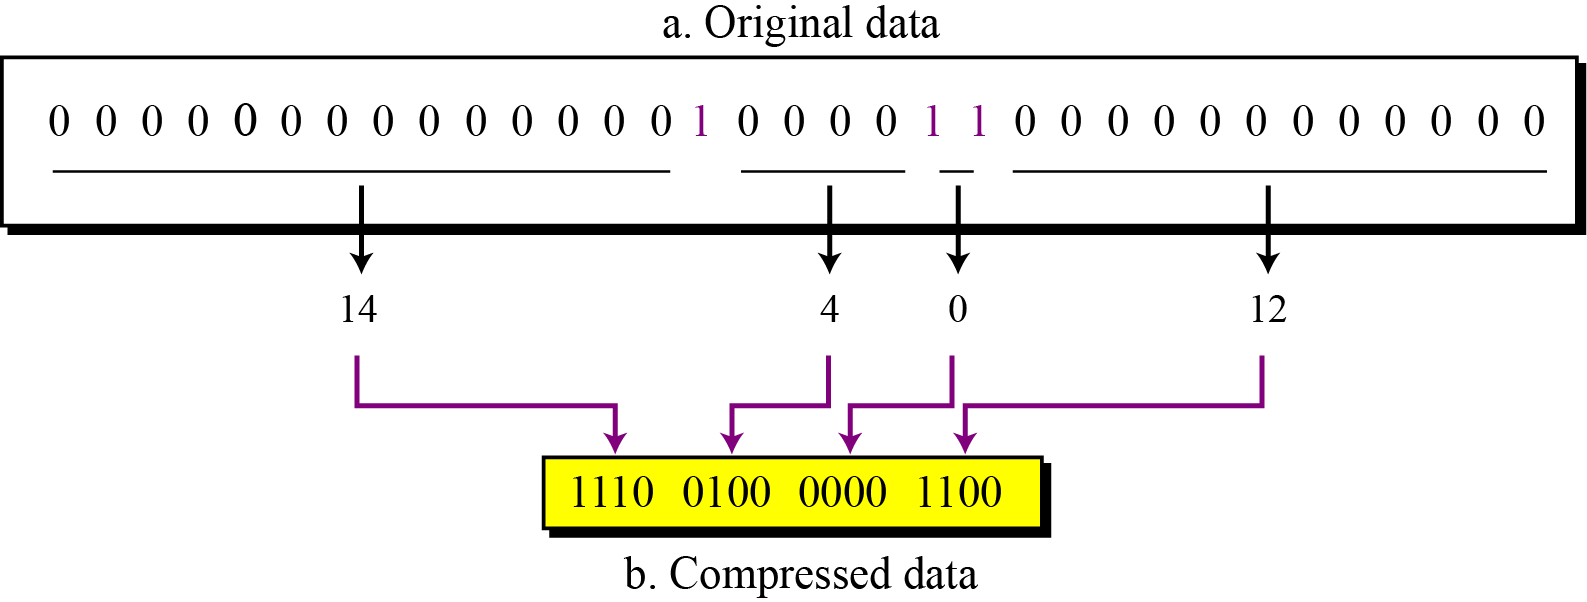
\includegraphics[width=\linewidth]{images/run_length_encoding.png}
  \caption{Run-Length Encoding Example}
\end{figure}

\subsection*{Huffman Coding}



% Original and coded input
\begin{table}[ht]
  \centering
  \resizebox{0.7\linewidth}{!}{%
    \begin{tabular}{ll}
      \toprule
      Original & \texttt{ABACABAD}       \\
      Encoded  & \texttt{01001100100111} \\
      \bottomrule
    \end{tabular}%
  }
  \caption{Original input and its Huffman-coded bitstream.}
  \label{tab:encoded}
\end{table}


% Frequency table
\begin{table}[ht]
  \centering
  \resizebox{0.5\linewidth}{!}{%
    \begin{tabular}{ll}
      \toprule
      Symbol & Frequency \\
      \midrule
      A      & 4         \\
      B      & 2         \\
      C      & 1         \\
      D      & 1         \\
      \bottomrule
    \end{tabular}%
  }
  \caption{Frequency table of input symbols.}
  \label{tab:freq}
\end{table}



\begin{figure}[ht]
\centering
\begin{forest}
for tree={
  circle,
  draw,
  minimum size=3em,
  inner sep=1pt,
  l=1.5cm,
  s sep=3cm,
  edge={thick},
  edge label/.append style={inner sep=1pt},
}
[{$8$}
  [{$A:4$}, edge label={node[midway,left,above=0.1cm]{$0$}}]
  [{$4$}, edge label={node[midway,right,above=0.1cm]{$1$}}
    [{$B:2$}, edge label={node[midway,left,above=0.1cm]{$0$}}]
    [{$2$}, edge label={node[midway,right,above=0.1cm]{$1$}}
      [{$C:1$}, edge label={node[midway,left,above=0.1cm]{$0$}}]
      [{$D:1$}, edge label={node[midway,right,above=0.1cm]{$1$}}]
    ]
  ]
]
\end{forest}
\caption{Huffman Tree for the Example}
\end{figure}
